\section{Conclusions}\label{conclusion_section}

This note has discussed the multiple coloumb scattering technique for estimating the momentum of a three dimensional reconstructed track and provided motivation for demonstration of the capabilities of this tool within the neutrino LArTPC community. The details of the implementation of this code have been described. The gaussian nature of scatters predicted by the Highland formula has been demonstrated. Additionally the performance of this method has been quantified in three different forms of simulation of fully contained tracks (single muon {\sc MCTracks}, truth-selected simulated BNB neutrino events, and automatically-selected selected BNB + cosmic neutrino events) as well as in approximately 0.5e20 POT of {\ub} data. The methods used to optimize the segment length (10 cm) and detector resolution term (2 mrad) in the MCS algorithm have been described. To summarize the performance on these different fully contained track samples, the bias and resolution for the different samples are overlaid in Figure \ref{MCS_range_bias_resolution_masteroverlay_fig}. Other uses besides momentum reconstruction for the MCS technique have been described, including using it as a tool for identification of poorly reconstructed tracks, determination of track direction, particle identification. 


\begin{figure}
\centering
\mbox{
	\subfigure[\textit{MCS momentum bias as a function of range momentum.}]
	{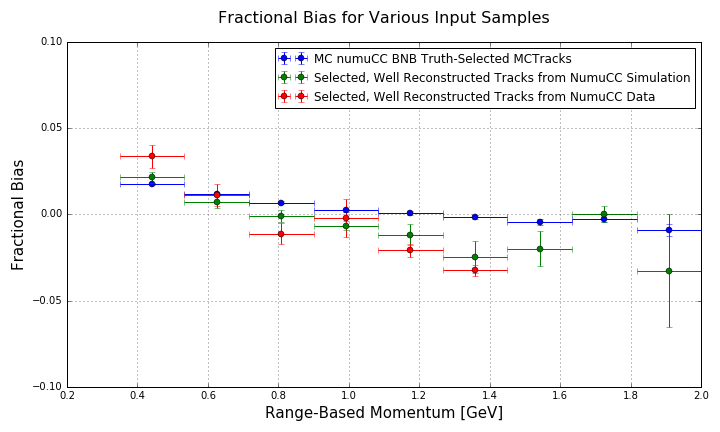
\includegraphics[width=80mm]{Figures/MCS_range_bias_multiplesamples.png}}
	\quad
	\subfigure[\textit{MCS momentum resolution as a function of range momentum.}]
	{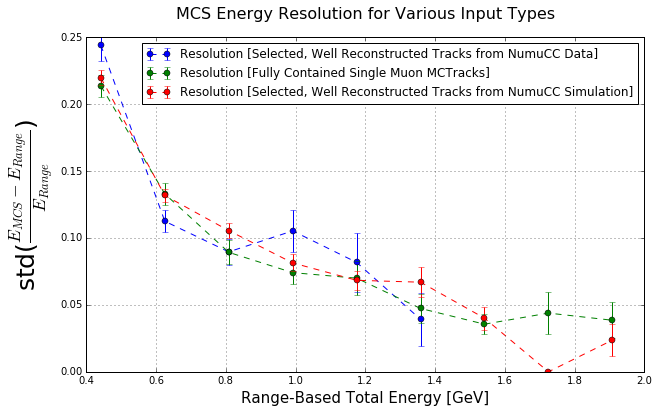
\includegraphics[width=80mm]{Figures/MCS_range_resolution_multiplesamples.png}}
	}
\caption{\textit{MCS Momentum resolution for simulated contained single muon {\sc MCTracks} discussed in Section \ref{singlemu_mctrack_performance_section} (blue), automatically selected contained numuCC-induced muons from simulated BNB+cosmics where the track is well-reconstructed and matches with the true muon track discussed in Section \ref{MC_performance_section} (green), and automatically selected contained numuCC-induced muons from MicroBooNE data where the track is deemed well-reconstructed and likely-muon from hand scanning discussed in Section \ref{data_performance_section}.}}
\label{MCS_range_bias_resolution_masteroverlay_fig}
\end{figure}












\section{Possible Plots for Publication}\label{publicplots_section}
Here are a few plots that I think should be considered for the publication. Bear in mind, in my opinion the publication should have its scope kept small so as to get it published in a very quick time scale. These plots of course can be modified, their captions changed, etc... I am just putting them here to paint a picture for the readers of this technote what I think should be included in the publication.
\begin{enumerate}
	\item Figure \ref{pub_plot_1} is a general image whose purpose is to aid the reader in understanding what MCS is and how the code works. I'm not sure this one is public-domain, but I can easily make my own version of it if necessary.
	\item Figure \ref{pub_plot_2} is an image whose purpose is to validate using range-based momentum in place of true-momentum when the analysis is done on real data where true-momentum obviously is unknown.
	\item Figure \ref{pub_plot_3} is an image showing the MCS momentum versus range momentum for the automatically selected, handscanned data events.
	\item Figure \ref{pub_plot_4} is an overlay of MCS momentum bias and resolution for various different types of inputs ({\sc MCTracks} in MC, reconstructed tracks in MC, reconstructed tracks in data). I'll note that since {\sc MCTracks} are sort of MicroBooNE specific, it is possible (and probably best) to leave them out of the publication entirely and therefore avoid having to describe them to readers.
\end{enumerate}

% Image describing MCS idea
\begin{figure}[ht!]
\centering
	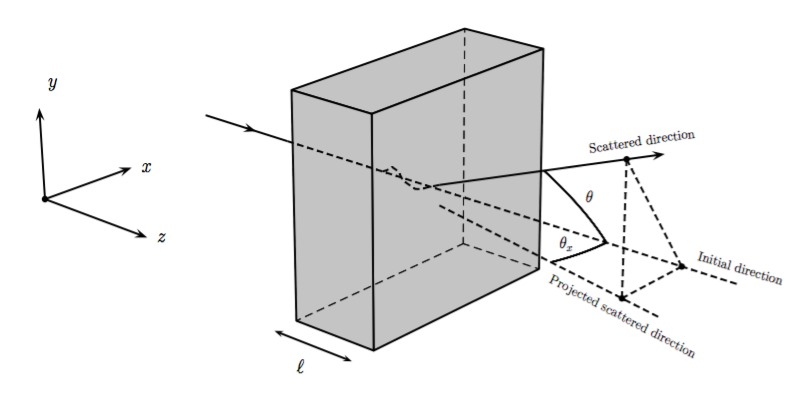
\includegraphics[width=0.5\linewidth]{Figures/mcs_nocap.png} \\
\caption{\textit{The particle's trajectory is deflected as it traverses through the material \cite{leonidas1}.}}\label{pub_plot_1}
\end{figure}

% Image validating range-based energy
\begin{figure}
\centering
\mbox{
	\subfigure[\textit{Range energy bias as a function of true energy.}]
	{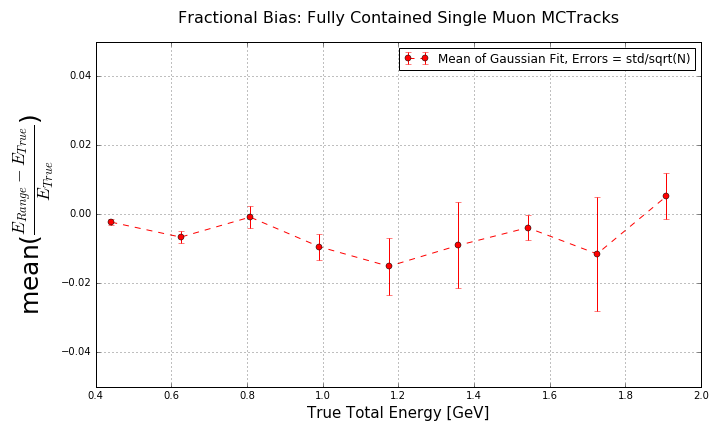
\includegraphics[width=75mm]{Figures/true_range_bias_SingleMuonMCTrack.png}}
	\quad
	\subfigure[\textit{Range energy resolution as a function of true energy.}]
	{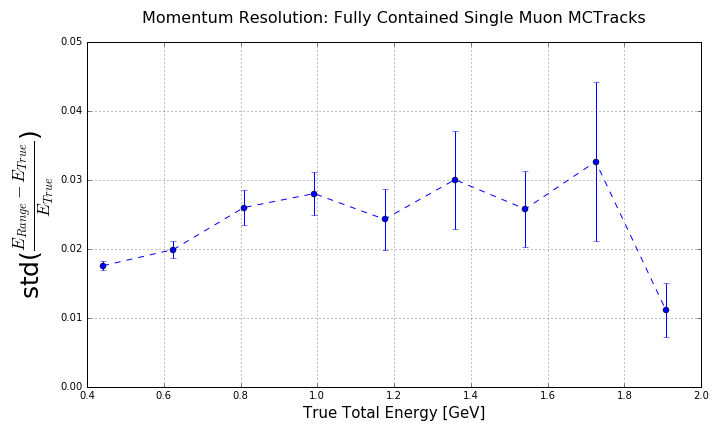
\includegraphics[width=75mm]{Figures/true_range_resolution_SingleMuonMCTrack.png}}
	}
\caption{\textit{Range energy and true energy bias and resolution for the single muon {\sc MCTrack} sample described in Section \ref{MCTrack_Selection_section}.}}
\label{pub_plot_2}
\end{figure}


% Image showing MCS momentum vs range momentum the handscanned data events
\begin{figure}
\centering
	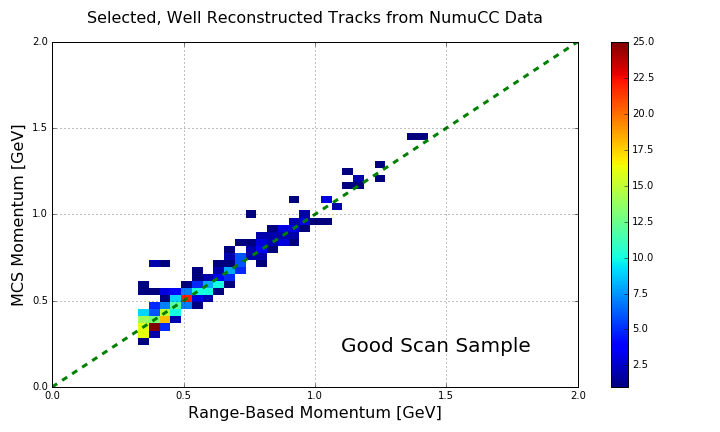
\includegraphics[width=75mm]{Figures/MCS_range_momentum_DataRecoTracks_goodhandscan.png}
\caption{\textit{MCS computed momentum versus range momentum for the selected neutrino-induced fully contained muon sample in data hand-scanned as having well reconstructed, likely-muon tracks.}}
\label{pub_plot_3}
\end{figure}


% Image showing bias and resolution for single mu MCTracks, auto selected neutrino in MC (truth muon only), auto selected neutrino in data (with handscan)

\begin{figure}
\centering
\mbox{
	\subfigure[\textit{MCS energy bias as a function of range energy.}]
	{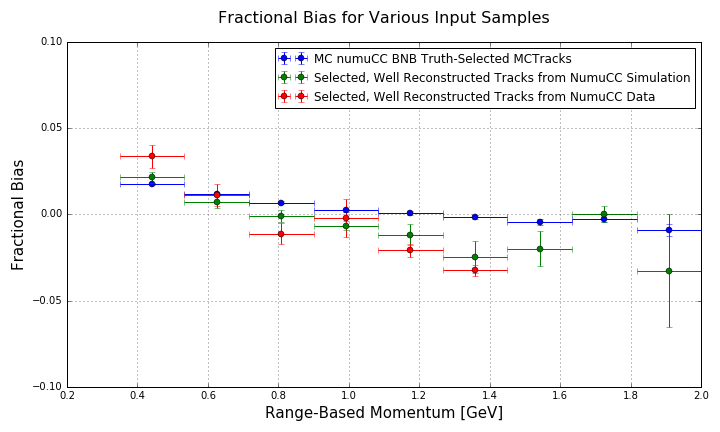
\includegraphics[width=80mm]{Figures/MCS_range_bias_multiplesamples.png}}
	\quad
	\subfigure[\textit{MCS energy resolution as a function of range energy.}]
	{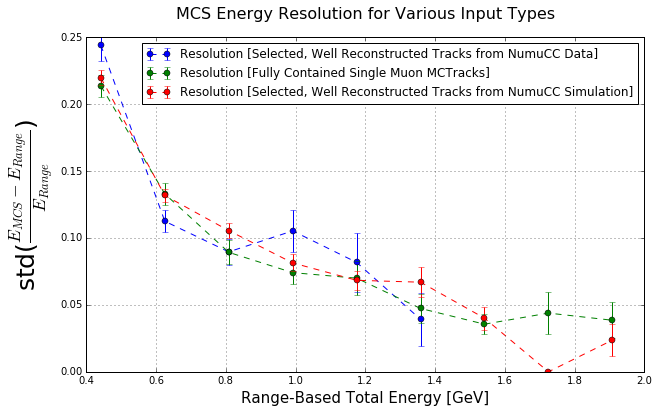
\includegraphics[width=80mm]{Figures/MCS_range_resolution_multiplesamples.png}}
	}
\caption{\textit{MCS Momentum resolution for simulated contained single muon {\sc MCTracks} discussed in Section \ref{singlemu_mctrack_performance_section} (blue), automatically selected contained numuCC-induced muons from simulated BNB+cosmics where the track is well-reconstructed and matches with the true muon track discussed in Section \ref{MC_performance_section} (green), and automatically selected contained numuCC-induced muons from MicroBooNE data where the track is deemed well-reconstructed and likely-muon from hand scanning discussed in Section \ref{data_performance_section}.}}\label{pub_plot_4}
\end{figure}

